\documentclass[a4j, 11pt]{jarticle}
%#DVIPDF dvipdfmx -f ipa.map
\addtolength{\topmargin}{-2cm}
\addtolength{\textheight}{4cm}
\addtolength{\textwidth}{2cm}
\addtolength{\oddsidemargin}{-2cm}
\usepackage{ascmac}
\usepackage{lineno}
\usepackage{graphicx}
\usepackage{multicol}
\usepackage{multirow} 
\pagestyle{empty}
\begin{document}
\vspace*{1em}


\begin{table}[t]
 \scalebox{1.1}[1.2]{
  \begin{tabular}{|l|c|c|c|c|c|}
   \cline{1-5}
   ふりがな & \multicolumn{4}{|p{26em}|}{ふりがなhogehoge}  & \multicolumn{1}{|c}{\multirow{5}{40mm}{
\begin{minipage}{30mm}
    \centering
    \scalebox{0.4}{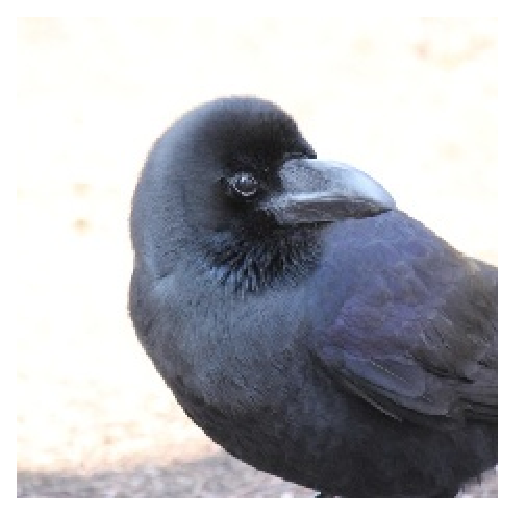
\includegraphics{./File/crow.eps}}
   \end{minipage}}} \\ \cline{1-5} 
   氏名 & \multicolumn{4}{|l|}{}\\

    & \multicolumn{4}{|l|}{\Large 荒木勇人}\\ \cline{1-5}

   生年月日 &  \multicolumn{3}{|c|}{1918-12-8} & 男 \\ \cline{1-5}

   電話番号 & \multicolumn{4}{|l|}{042(443)5102}  \\ \cline{1-5}
   E-mail & \multicolumn{4}{|l|}{hogehogehoge@cs.euc.ac.jp}  \\ \hline

   ふりがな & \multicolumn{4}{|l|}{ふりがなhogehoge juusho 1-5-1} & 電話 \\ \cline{1-5}

    郵便番号〒 & \multicolumn{4}{|l|}{182-8585} & \multirow{2}{*}{042(443)5102}\\ 
     & \multicolumn{4}{l|}{kanji juusho} & \\ \hline

   ふりがな & \multicolumn{4}{|l|}{} & 電話 \\ \cline{1-5}
   連落先〒 & \multicolumn{4}{|l|}{(現住所以外に連絡を希望する場合のみ記入)} & \multirow{2}{*}{042(443)5102} \\
   & \multicolumn{4}{|l|}{} & \\
   \hline
  \end{tabular}
}

\end{table}


\section{araki-t@mm.inf.uec.ac.jp}
\end{document}